% Vorbereitung: Vorbereitungsaufgaben bearbeiten
% Versuchsaufbau: Verwendete Apparatur, Beschreibung Funktionsweise/Nutzen mit Skizze/Foto
\section{Durchführung}
\label{sec:durchführung}

Im Folgenden wird der Versuchsaufbau erklärt und die Messdurchführung wird beschrieben.

\subsection{Versuchsaufbau}
\label{sec:Versuchsaufbau}
Die \autoref{fig:bild4} zeigt die transparente Grundplatte, welche zur Untersuchung der grundlegende Gesetzmäßigkeiten der Strahlenoptik und der Wellenoptik
verwendet wird.
\begin{figure}[H]
    \centering
	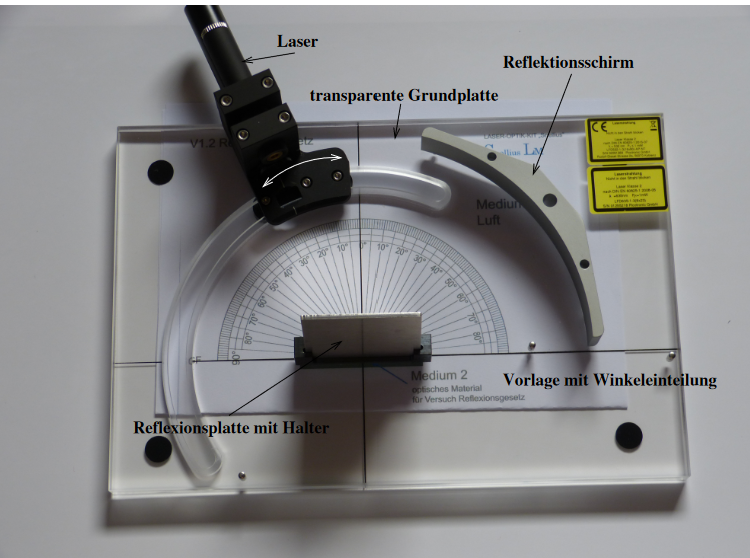
\includegraphics[width=0.6\linewidth]{content/grafik/aufbau.png}
	\caption{Transparente Grundplatte auf der sich zwei Laserdiodenmodule befinden. \cite{reflex}}
	\label{fig:bild4}
\end{figure}
Auf der Platte befinden sich zwei Laserdiodenmodule, welche Licht mit der Wellenlänge $\lambda_{\text{rot}} = \SI{635}{\nano\meter}$ und
$\lambda_{\text{grün}} = \SI{532}{\nano\meter}$ emittieren. Diese Laserdioden lassen sich im Halbkreis bewegen.
In der Mitte  des Halbkreises lassen sich für die unterschiedlichen Versuchsaufgaben verschiedene geometrische Elemente einbauen.

\subsection{Versuchsaufgabe}
\label{sec:Versuchsaufgaben}

Zunächst wird das Reflexionsgestz untersucht, indem der gründe Laser, die Vorlage a und der Halter mit dem Spiegel verwendet werden.
Für 7 Einfallswinkel $\alpha_1$ werden die Ausfallswinkel $\lambda_2$ gemessen.

Als Zweites wird das Brechungsgesetz untersucht, dafür wird der Brechungsindex von Luft $n_1 = 1$ genähert.
Verwendet werden der grüne Laser, die Vorlage a und die planparallele Platte. Die Platte wird so positioniert, dass 
der Eintrittsspalt zur Winkelskala zeigt. Die \autoref{fig:bild5} zeigt den Prozess, bei dem der Lichtstrahl durch eine planparallele
Platte geht und dabei zwei Brechungen erfährt.
\begin{figure}[H]
    \centering
	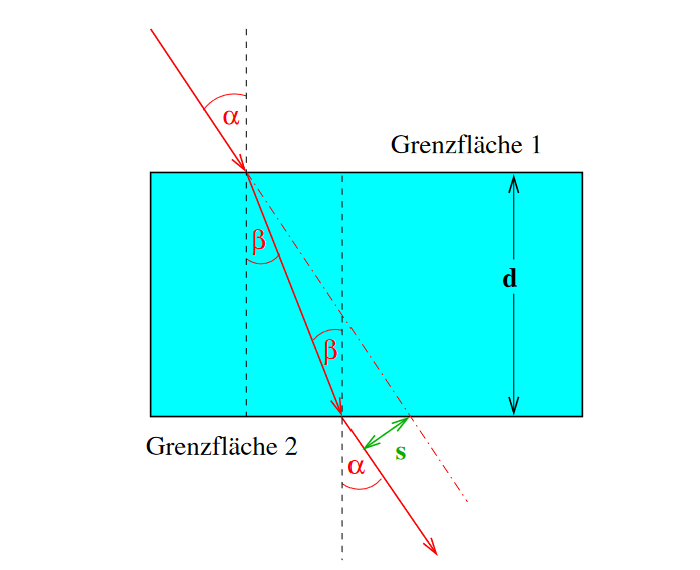
\includegraphics[width=0.6\linewidth]{content/grafik/strahlen.png}
	\caption{Strahlenversatz an einer planparallelen Platte. \cite{reflex}}
	\label{fig:bild5}
\end{figure}
Der Strahlenversatz $s$ lässt sich berechnen über die Gleichung 
\begin{equation}
	s=d \frac{\sin (\alpha-\beta)}{\cos \beta}.
	\end{equation}
Bestimmt wird der Brechungswinkel $\beta$ für 7 verschiedene Einfallswinkel $\alpha$.

Ein optisches Prisma wird durch nicht parallele Flächen begrenzt. Trifft ein Lichtstrahl in das Prisma ein,
nennt man die beiden Grenzflächen, welches der Lichtstrahl durchläuft, brechende Kanten. Diese begrenzen den brechenden Winkel 
$\gamma$ des Prismas. Die \autoref{fig:bild6}  zeigt ein solches optisches Prisma.
\begin{figure}[H]
    \centering
	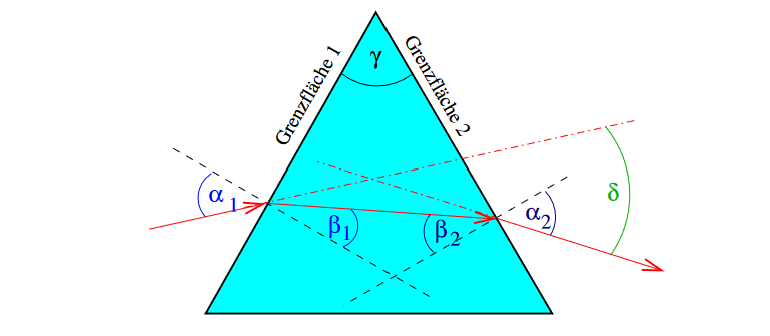
\includegraphics[width=0.6\linewidth]{content/grafik/prisma.png}
	\caption{Optisches Prisma. \cite{reflex}}
	\label{fig:bild6}
\end{figure}
Die Ablenkung $\delta$, die der Strahl beim Durchgang durch das Prisma erfährt, lässt sich über 
\begin{equation}
	\delta = \left(\alpha_1 + \alpha_2\right) - \left(\beta_1 + \beta_2\right)
\end{equation}
berechnen.
Es werden alle Messungen sowohl für den grünen als auch für den roten Laser durchgeführt. Verwendet wird die Vorlage c
und das Prisma. Für jeweils 5 verschiedene Einfallswinkel $\alpha_1$ im Bereich von $\qty{30}{°}$ bis $\qty{80}{°}$ werden die Ausfallswinkel $\alpha_2$ gemessen.

Zum Schluss werden in die Halterung drei verschiedene Gitter eingesetzt. Dabei ist es drauf zu achten, dass das Laserlicht die Winkelskala
des Transmissionsschirms bei $\qty{0}{°}$ trifft und dass der Transmissionsschirm im Kreis um die Winkelskala der Vorlage angeordenet ist.
Die Ablenkwinkel $\gamma$ werden so direkt abgelesen. Die Gitterkonstanten der drei Gitter sind in \autoref{sec:Vorbereitungsaufgabe} angegeben.

\section{Vorbereitungsaufgabe}
\label{sec:Vorbereitungsaufgabe}

In der \autoref{tab:brechungs} sind die Brechungsindizes verschiedener Materialien aufgelistet. 
\begin{table}[H]
	\centering
	\caption{Brechungsindizes}
	\label{tab:brechungs}
\begin{tabular}{c c}
	\toprule
	Material & Brechungsindex \\
	\midrule
	Luft & 1.000922 \\
	Wasser & 1.333 \\
	Kronglas & 1.510 \\
	Plexiglas & 1.49 \\
	Diamant & 2.417 \\
	\bottomrule
\end{tabular}
\end{table}

Für die drei verwendeten Gitter wurden die Gitterkonstanten berechnet und in \autoref{tab:gitter} dargestellt.
\begin{table}
    \centering
    \caption{Gitterkonstanten $d$ der drei Gitter.}
	\label{tab:gitter}
    \begin{tabular}{c c}
        \toprule
        Gitter $\mathbin{/}\unit{\frac{\newton}{\milli \meter}}$& Gitterkonstante $d$ $\mathbin{/} \symup{mm}$\\
        \midrule
        600& 0.00167\\
        300 & 0.00333\\
        100 & 0.00100\\
        \bottomrule
    \end{tabular}
\end{table}